\documentclass[12pt]{article}
 
\usepackage[margin=1in]{geometry} 
\usepackage{amsmath,amsthm,amssymb, mathtools}
\usepackage{multicol}
\usepackage[subnum]{cases}
\usepackage{relsize}
\usepackage[makeroom]{cancel}
\usepackage[english]{babel}
\usepackage{graphicx}
\usepackage{calligra}
\usepackage[normalem]{ulem}
\usepackage{caption}
\usepackage{subcaption}
\usepackage{siunitx}
\usepackage{ mathrsfs }
\usepackage{float}
\usepackage{hyperref}
\usepackage{url}
\usepackage[font={footnotesize}]{caption}


\DeclareMathAlphabet{\mathcalligra}{T1}{calligra}{m}{n} 
\DeclareFontShape{T1}{calligra}{m}{n}{<->s*[2.2]callig15}{}


% Makes '\sr' make a script r
\newcommand{\sr}{\ensuremath{\mathcalligra{r}}}
 
\newcommand{\N}{\mathbb{N}}
\newcommand{\Z}{\mathbb{Z}}
\newcommand{\ihat}{\boldsymbol{\hat{\textbf{\i}}}}
\newcommand{\jhat}{\boldsymbol{\hat{\textbf{\j}}}}
\newcommand{\khat}{\boldsymbol{\hat{\textbf{k}}}}
\newcommand{\rhat}{\boldsymbol{\hat{\textbf{r}}}}
\newcommand{\srhat}{\boldsymbol{\hat{\textbf{\sr}}}}
\newcommand{\xhat}{\boldsymbol{\hat{\textbf{x}}}}
\newcommand{\yhat}{\boldsymbol{\hat{\textbf{y}}}}
\newcommand{\zhat}{\boldsymbol{\hat{\textbf{z}}}}
\newcommand{\phihat}{\boldsymbol{\hat{\textbf{$\phi$}}}}

\newcommand{\vect}[1]{\boldsymbol{\vec{#1}}}
\newcommand{\fracl}[2]{\mathlarger{\frac{#1}{#2}}}
\newcommand{\dd}{\, \mathrm{d}}
\newcommand{\eo}{\epsilon_\circ}
\newcommand{\mo}{\mu_\circ}
\newcommand{\tder}[2]{\frac{\dd #1}{\dd #2}}
\newcommand{\pder}[2]{\frac{\partial #1}{\partial #2}}
\newcommand{\dtder}[2]{\frac{\dd^2 #1}{\dd #2^2}}
\newcommand{\dpder}[2]{\frac{\partial^2 #1}{\partial #2^2}}
\newcommand{\intas}{ \int_{-\infty}^\infty}
\newcommand{\npar}{\\[0.5cm] \noindent}


\begin{document}

\title{Engineering and Computational Techniques of Particle Detection Utilized in the Compact Muon Solenoid}
\author{Roy Smart \\ Montana State University \\PHSX 451 Elementary Particle Physics}
\maketitle

\section{Introduction}
On July 4th 2012, CERN hosted a press conference to announce their findings from the Large Hadron Collider (LHC) \cite{website:higgs_press}. While the world waited with baited breath, CERN researchers confirmed they had identified a new particle with mass 125 GeV. Furthermore this particle decayed into two photons, indicating that the new particle was a boson with a spin not equal to one\cite{new_higgs}.  This information implied the existence of the Higgs boson, a particle that has been postulated to exist for at least 60 years \cite{higgs_predict}. 
\npar
The LHC utilizes two complementary general-purpose detectors: ATLAS (A Toroidal LHC ApparatuS) and CMS (Compact Muon Solenoid). The two detectors work independently of one another, and in the case of the Higgs particle, provide independent verification of discovery \cite{lhc_combo}. In this paper, we present a small portion of the data presented by the CMS collaboration that supports the existence of a Higgs boson with mass 125 GeV. We will then explore the engineering strategies of the CMS detector that enabled this unique discovery, and the computational techniques used to validate the possible existence of the Higgs.


\section{CMS Collaboration Results}
\subsection{Interpreting CMS Data}
The existence of the Higgs boson can not be detected directly, rather it is identified through its decay products \cite{higgs_search}. These decay products are not only produced in the Higgs decay, but are created through the decay of other particles. The decay products produced in reactions of previously discovered particles are known as the ``background'' and the search for the Higgs must show that the rates of the pertinent decays are significantly higher than the background rates of decay.
\npar
 The mass of the Higgs was unknown prior to the experiment, so the CMS collaboration elected to analyze the so-called low-mass region ($m_H = 110-160 \; \text{GeV}$, where $m_H$ is the invariant mass of the Higgs boson) their search for the Higgs. To identify the Higgs, the CMS collaboration selected five of the decay modes that their detector was most sensitive to. Experiment parameters such as the production cross section, branching ratios, particle identification efficiency, mass resolution, and the amount of background signal from similar processes were all considered to identify the decay modes that would provide the most sensitivity. Two decay modes provided high mass resolution: $H\rightarrow \gamma \gamma$ and $H \rightarrow ZZ \rightarrow 4\ell$; while three other modes only provided low mass resolution: $H \rightarrow WW \rightarrow 2\ell2\nu$, $H \rightarrow \tau \tau$ followed by at least one leptonic $\tau$ decay, and $H \rightarrow bb$ followed by b-quark fragmentation into jets. The $ZZ$ and $\gamma \gamma$ modes are important because of the experiment parameters stated above, they provide a excellent resolution (1-2 GeV) of the invariant mass of the decay products, and consequently give the best estimate for the value of the Higgs' mass \cite{new_higgs}. For the remainder of this paper we will be exploring the CMS collaboration's analysis of the $H \to ZZ$ decay mode, and specific technical information as to how their result was calculated.
\subsection{The $H \to ZZ$ Decay Mode}
The Higgs has two fully leptonic decay modes
\begin{align}
 &H \to WW \to \ell^+\nu \; \ell^- \; \overline{\nu}
\intertext{and}
&H \to ZZ \to \ell^+ \ell^- \ell^+ \ell^- \label{golden}
\intertext{where}
& \ell = [e \; (\text{electron}), \; \mu \; (\text{muon})] \quad \text{and} \quad \nu = (\text{neutrino}) \nonumber
\end{align}
The first decay mode is non-ideal since the neutrinos cannot be detected, rather their presence is inferred by noting the energy missing after a reaction\cite{new_higgs}. However, the decay mode (\ref{golden}) is known as the `golden' channel for discovery.  This is due to the fact that the entire decay chain can be fully reconstructed with high resolution \cite{higgs_hunt} because the invariant mass of the electron and muon decay products are easily resolved by the CMS detector \cite{golden_higgs}. Due to their short lifetimes, the tauons are not considered as they decay into smaller particles before interacting with the CMS. The high resolution of the golden channel compared to other decay modes comes with a price: the branching ratio of the $ Z \to \ell^+ \ell^- $ is only 3.37\%, so only a small amount of the Higgs bosons which decay via the $ZZ$ channel will decay further into the golden channel\cite{higgs_hunt}. Another challenge that presents itself is the background signals from quark-antiquark and gluon-gluon processes produce quantitatively similar events, further obscuring possible Higgs detections \cite{new_higgs}. \npar

\begin{figure}[h!]
\centering
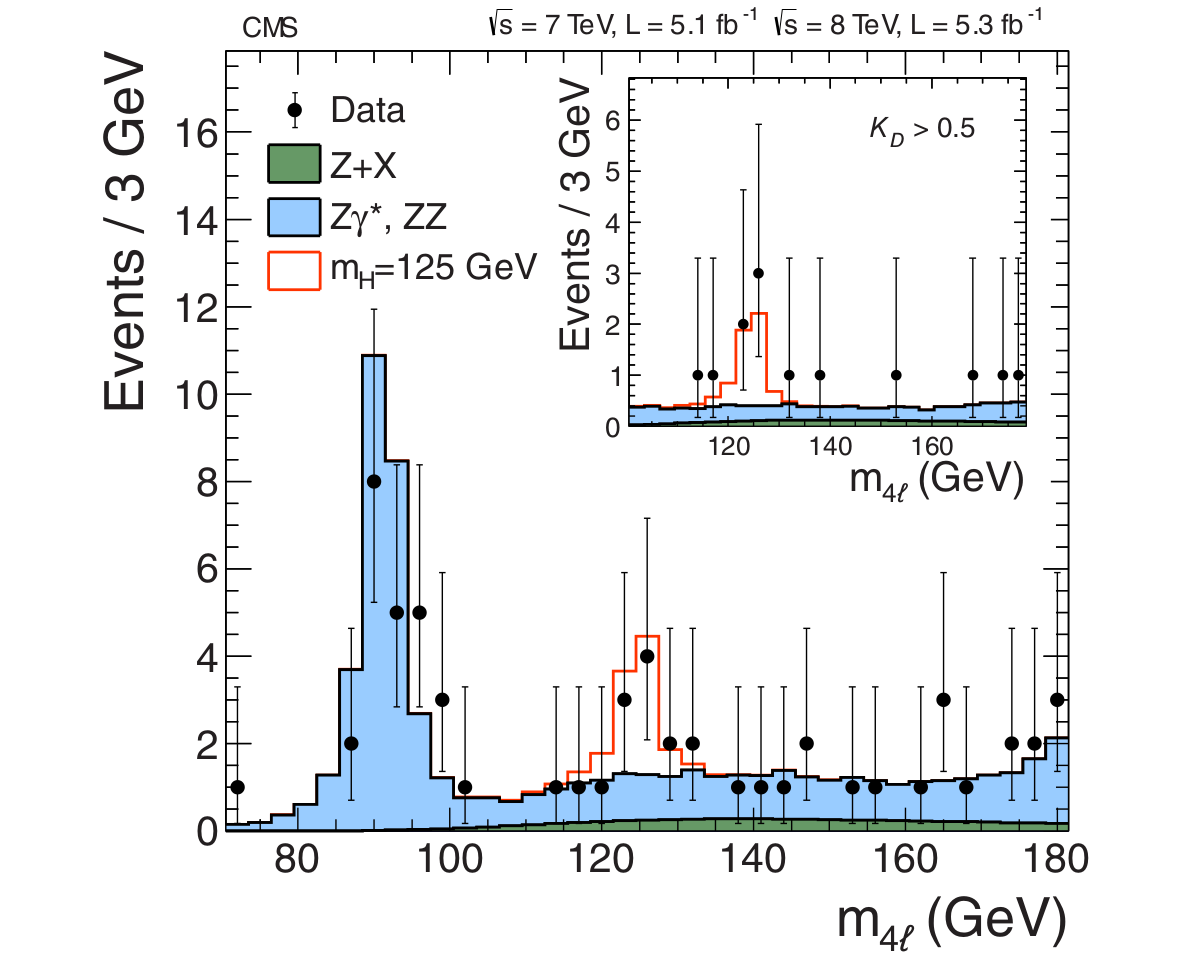
\includegraphics[width=0.8\textwidth]{images/HtoZZ}
\caption{Distribution depicting the four-lepton invariant mass for the CMS collaboration's $ZZ \to 4 \ell$ analysis. The points represent data gathered by the CMS experiment, the filled histograms represent the predicted four-lepton background signal, and the red histogram represents the predicted four-lepton signal for the Higgs boson with a mass of 125 GeV. The inset distribution represents the same plot after the background events have been minimized.}
\label{HtoZZ}
\end{figure}
\noindent
The data we will be discussing is provided in Figure \ref{HtoZZ}, which depicts the evidence supporting a Higgs boson with mass of 125 GeV via the $ZZ$ channel. Figure \ref{HtoZZ} shows the measured data overlaid on both the predicted background signal from processes unrelated to Higgs production and the predicted signal of a Higgs boson with mass 125 GeV. The inset to Figure \ref{HtoZZ} displays only data for which the value of the kinematic discriminant, $K_D$, is greater than 0.5 where
\begin{align*}
K_D = \frac{\mathcal{P}_{sig}}{\mathcal{P}_{sig} + \mathcal{P}_{bkg}}  &> 0.5 \quad \cite{new_higgs}\\
\Rightarrow 2\mathcal{P}_{sig} &> \mathcal{P}_{sig} + \mathcal{P}_{bkg} \\
\Rightarrow \mathcal{P}_{sig} &> \mathcal{P}_{bkg}.
\end{align*}
$\mathcal{P}_{sig}$ is the probability that a measurement represents a Higgs signal and $\mathcal{P}_{bkg}$ is the probability that a measurement represents a background process \cite{recent_results}. The methods used to determine these probabilities will be discussed later in this document.

\subsection{Determining the Invariant Mass of the 4-Lepton Products from CMS Measurements}

To determine the invariant mass of the lepton products, $m_{4 \ell}$, plotted on the horizontal axis of Figure \ref{HtoZZ}, the CMS Collaboration had to first identify four valid leptons, reconstruct their energy and momentum, and then use relativistic kinematics to evaluate the invariant mass of the system. This process is described in detail by  To identify the first lepton pair, the CMS trigger system selects collision events that produce a pair of leptons with transverse energy for the first and second lepton above 17 and 8 Gev respectively. Electrons are identified within the transverse momentum range $p_T > \SI{7}{GeV}$ and the the pseudorapidity range of $|\eta| < 2.5$, where $\eta = \ln[\tan(\theta/2)]$ and $\theta$ is the polar angle with respect to the direction of the proton beam. Muons are reconstructed within the range $|\eta| < 2.4$ and $p_T > \SI{5}{GeV}$. The pseudorapidity ranges for electrons and muons are determined by the sensitivity of the ECAL and the muon return yoke for a given $\eta$ Furthermore, to ensure an accurate measurement, the leptons are required to be isolated by requiring the sum of the transverse momenta of tracks $i$ in a cone of radius $\Delta R = \sqrt{(\eta^\ell - \eta^i)^2 + (\phi^\ell - \phi^i)^2} < 0.3$ where $\phi$ is the azimuthal angle, to be $\sum_ip_T^i/p_\ell < 0.7$ \cite{higgs_golden_search}. \npar
For the first $Z$ candidate the CMS collaboration required that it be formed with a pair of lepton candidates satisfying $50 < m_{1,2} < \SI{120}{GeV}$, where
\begin{align}
	mc^2 &= \sqrt{E^2 - \mathbf{p}^2c^2} \quad \cite{griffiths}
\end{align}
and $E$ is the total energy and $\mathbf{p}$ is the total three-momentum of the lepton products. To ensure that the leptons are in the high-efficiency region for the trigger, there is the additional constraint that the transverse momentum of the first lepton is greater than 20 GeV and the second is greater than 10 GeV. From these candidates, the $Z$ boson closest to the reconstructed mass is denoted $Z_1$. This defines the $Z_1 + X$ dataset, which is used to eliminate background measurements.
For the signal measurement, another lepton pair with the same flavor and opposite charge is selected from the $Z_1 + X$ dataset and denoted $Z_2$. The CMS Collaboration required that the invariant mass of $Z_2$ must be greater than 12 GeV, with an additional restriction that the invariant mass of all four leptons must be at least 100 GeV.


The CMS collaboration identified several processes that can minimize the contribution of the background signals. While the quark-antiquark and gluon-gluon processes are impossible to remove because of their similarity to the golden channel, there are several background signals that can be minimized\cite{new_higgs}:
\begin{align}
& Z + b \overline{b}, \\
& Z + t \overline{t}, \\
& Z + \text{jets}, \\
\text{and} \qquad & WZ + \text{jets} .
\end{align}
The strategies for eliminating these background processes will be further discussed in Section \ref*{comp_tech}.
\npar
The invariant masses of the lepton products is determined using relativistic kinematics. The kinematics of the $H \to ZZ \to 4 \ell$ system can be solved completely in the rest frame of the Higgs using only seven parameters: the invariant masses of the lepton pairs and five angles \cite{new_higgs}, known as Cabibbo-Maksymowicz (CM) angles\cite{higgs_angles}. These angles are defined in Table \ref{angle_table} and Figure \ref{angle_fig}. It is interesting to note that the CMS collaboration did not consider the momentum of the $ZZ$ system, due to the dependence on the production mechanism and the additional complications of modeling the QCD effects\cite{new_higgs}. \\ \\
\begin{table}[h!]
\centering
\begin{tabular}{|c|l|}
\hline
Angle & Description \\ \hline \hline
$\Theta$ & The polar angle of the initial-state partons (gluons, quarks) in the H rest frame. \\ & Measured from the positive z axis (along the anti-clockwise beam direction) \\ \hline
$\theta_1$ & The polar decay angle of the $\ell_1^-$ in the $Z_1$ rest frame. \\ \hline
$\phi_1$ & The azimuthal decay angle of the $\ell_1^-$ in the $Z_1$ rest frame. \\ \hline  
$\theta_2$ & The polar decay angle of the $\ell_2^-$ in the $Z_2$ rest frame. \\ \hline
$\phi_2$ &  The azimuthal decay angle of the $\ell_2^-$ in the $Z_2$ rest frame. \\ \hline
\end{tabular}
\caption{The five Cabibbo-Maksymowicz angles in the $H \to ZZ$ decay mode, and their definitions \cite{higgs_angles}.}
\label{angle_table}
\end{table}

\begin{figure}[h!]
\centering
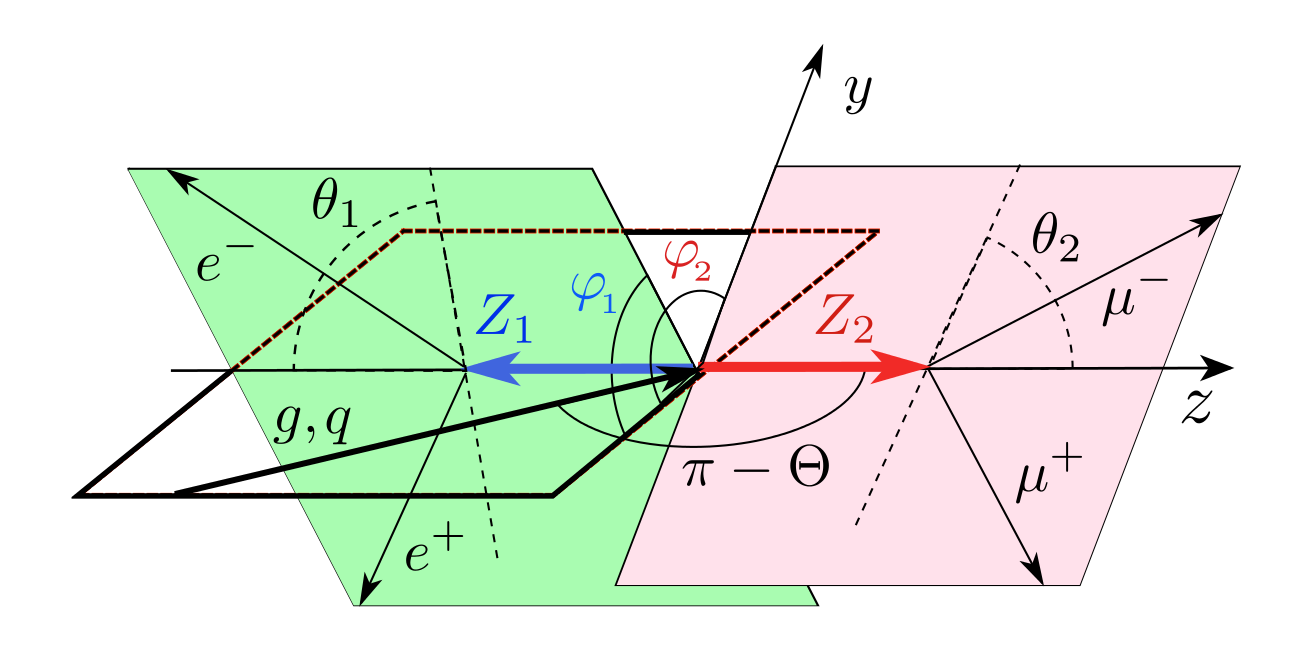
\includegraphics[width=0.7\textwidth]{images/HtoZZ_angles}
\caption{Visual description of the Cabibbo-Maksymowicz angles in the $H \to ZZ$ decay mode \cite{higgs_angles}.}
\label{angle_fig}
\end{figure}
\noindent
Armed with an understanding of the parameters associated with identifying the Higgs boson via the $H \to ZZ \to 4 \ell$ decay mode, we can now explore the design of the CMS experiment and identify what techniques are used to capture this data.

\section{Design of the Compact Muon Solenoid}

\begin{figure}[H]
\centering
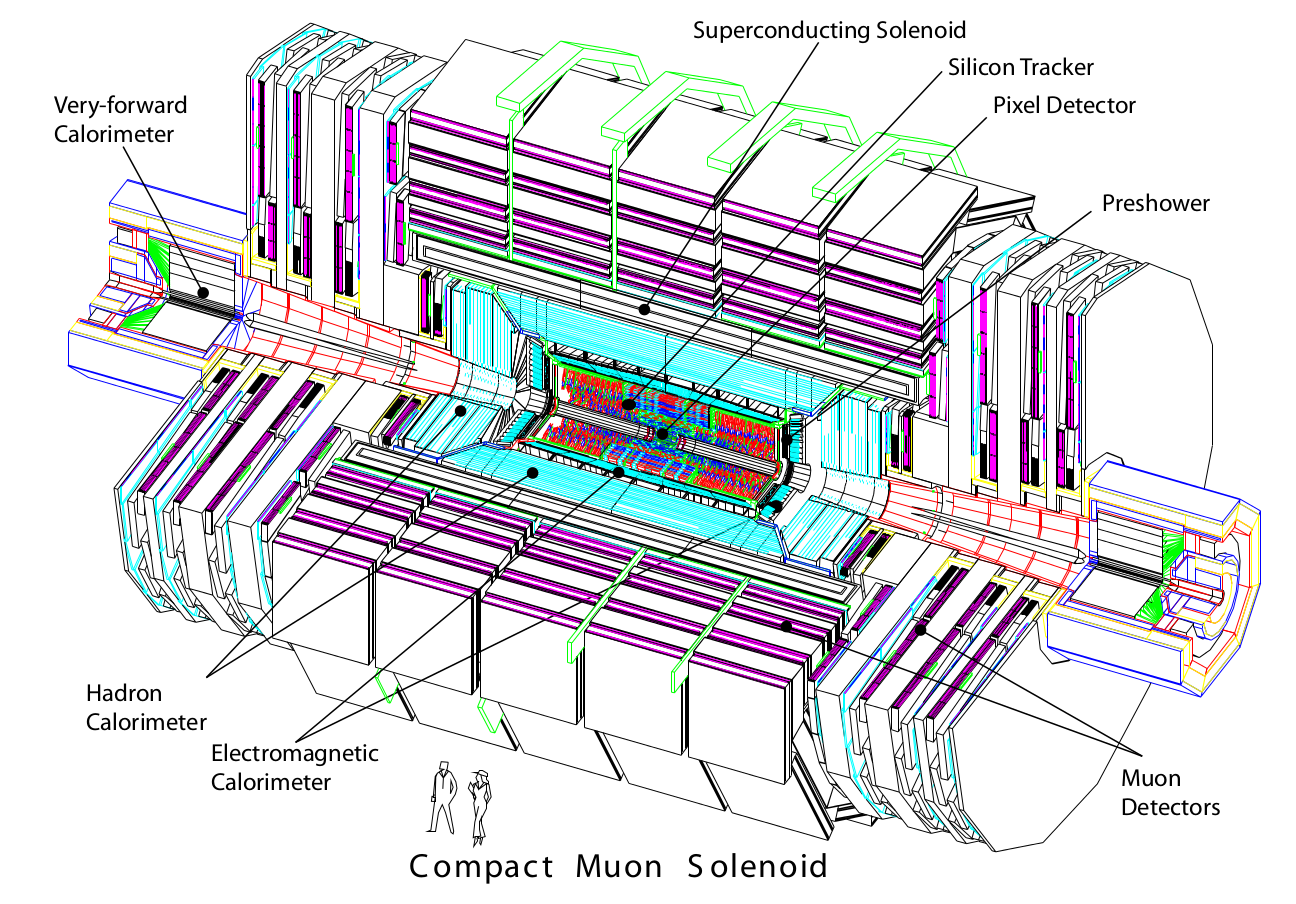
\includegraphics[width = 0.85\textwidth]{images/cms_persp}
\caption{A cut-away perspective view of the CMS experiment, with each of the major sensors within the experiment identified \cite{cms_design}.}
\label{cms_persp}
\end{figure}

\subsection{Overview}
The CMS experiment is designed to identify approximately 1000 charged particles emerging from the interaction region every 25ns. To ensure that the products of a single interaction are interpreted separately and that two subsequent interaction events don't get confused with one another, the experiment must use high-granularity detectors with good time resolution. This results in a large number of detector channels with very low occupancy, which produce an unprecedented amount of data. With these challenges in mind, the requirements of the experiment are as follows:
\begin{itemize}
\item Good muon identification and momentum resolution, with the ability to determine the charge of the muon.
\item Good charged-particle momentum resolution.
\item Good electromagnetic energy resolution, with the ability to isolate photons and leptons.
\item Good missing-transverse-energy and dijet-mass resolution.
\end{itemize}
\noindent
The heart of the CMS experiment is the superconducting solenoid, which is sandwiched between the calorimeters on the interior of the experiment, and the muon detectors on the exterior\cite{cms_design}. The solenoid provides a substantial magnetic field of 4T which is used to determine the momentum of charged particles and muons \cite{physics_requirements}. 
\npar
For analyzing the trajectories of leptons produced in the golden decay channel, data from nearly all of the sensors in the CMS experiment must be employed\cite{cms_tdr}.
\subsection{Tracker}
\subsection{Electromagnetic Calorimeter}
\subsection{Muon Detectors}


\section{Computational Techniques}
\label{comp_tech}
\subsection{CMS Software Architecture}
\subsection{Event Filter}
\subsection{Detector Description}
\subsection{Simulation}
\subsection{$H \to 4 \ell$ Analysis Code}
\section{Conclusion}



\bibliographystyle{unsrt}
\bibliography{sources}

\section{Questions for first draft}
\begin{enumerate}
\item Should the sources be organized in the order they were cited, or by author's last name?
\item In this paper, particles are identified in italics because \LaTeX \; automatically italicizes characters in math mode. Is this standard notation, or should I make an effort to unitalicize particle symbols?
\item I feel as if I am following the CMS collaborations paper, "Observation of a New Boson at a Mass of 125 Gev with the CMS Experiment at the LHC" too closely, as I have to cite it often. Is this inappropriate for this assignment? Is there a slight modification I can make to my topic to ensure that I don't just restate the work of the CMS collaboration, or is such a situation unavoidable when doing a research paper such as this?
\item Is it proper to cite source code in this context? I'm not quite sure I want to do that yet, but do you have any experience in these matters?


 
\end{enumerate}
\section{Other Remarks}
\begin{enumerate}
\item For convenience, a copy of all the sources I cited is available at \url{https://github.com/byrdie/PHSX_451_final_paper/tree/master/sources}
\item Please let me know if I am straying too far into Jackson Remington's territory on this project. I have been communicating with him, and it seems that he is focusing more on the theoretical side. If you find that our topics are overlapping by too much I would be happy to modify my paper to avoid redundancy.
\end{enumerate}


\end{document}